\باب{تفرق کا استعمال}
اس باب میں ہم تفرق سے نتائج اخذ کرنا سیکھیں گے۔ ہم تفرق کی مدد سے تفاعل کی انتہائی قیمتیں حاصل کرتے ہوئے ان کی ترسیم کی اشکال کی پیش گوئی کرتے ہیں اور ان پر تجزیہ کرتے ہیں، پیچیدہ کلیات کی سادہ صورت اخذ کرتے ہیں، تفاعل کی پیمائشی خلل کو حساسیت پر غور کرتے ہیں اور تفاعل کی صفر کو اعدادی طریقوں سے حاصل کرتے ہیں۔مسئلہ اوسط قیمت ان تمام کو ممکن بناتا ہے جس کا ایک منطقی نتیجہ تکملی احصاء کی راہ ہموار کرتا ہے۔  

\حصہ{تفاعل کی انتہائی قیمتیں}
اس حصہ میں استمراری تفاعل کی انتہائی قیمتوں کا مقام اور اور ان کی پہچان سکھائی جائے گی۔

\جزوحصہء{مسئلہ کم سے کم اور زیادہ سے زیادہ}
بند دائرہ کار کے ہر نقطہ پر استمراری تفاعل کا اس دائرہ کار پر مطلق بلند تر قیمت اور مطلق کم سے کم قیمت ہو گا جن پر ترسیم کھینچتے وقت  نظر رکھا جاتا ہے۔ مسائل کے حل میں ان انتہائی قیمتوں  کے کردار پر اس باب میں  جبکہ تکمل احصاء کی  نظریہ مرتب کرنے میں ان کے کردار پر اگلے دو ابواب میں غور کیا جائے گا۔  

\ابتدا{مسئلہ}\شناخت{مسئلہ_استعمال_بلند_تر_کمتر}\موٹا{استمراری تفاعل کا مسئلہ کم سے کم اور زیادہ سے زیادہ}\\
بند دائرہ کار \عددی{I} کے ہر نقطہ پر استمراری تفاعل \عددی{f} کا \عددی{I} پر مطلق زیادہ سے زیادہ قیمت \عددی{M} اور مطلق کم سے کم  قیمت \عددی{m} پایا جائے گا۔یعنی \عددی{I} میں ایسا \عددی{x_1} اور \عددی{x_2} پایا جائے گا کہ \عددی{f(x_1)=m} اور \عددی{f(x_2)=M} ہوں اور \عددی{I} میں تمام \عددی{x} کے لئے \عددی{m\le f(x)\le M} ہو (شکل \حوالہ{شکل_استعمال_بلند_تر_کم_تر})۔
\انتہا{مسئلہ}
%===================
درج بالا مسئلے کے ثبوت کے لئے حقیقی اعدادی نظام کا تفصیلی علم ضروری ہے لہٰذا اس کا ثبوت پیش نہیں کیا جائے گا۔ 
\begin{figure}
\centering
\begin{subfigure}{0.5\textwidth}
\centering
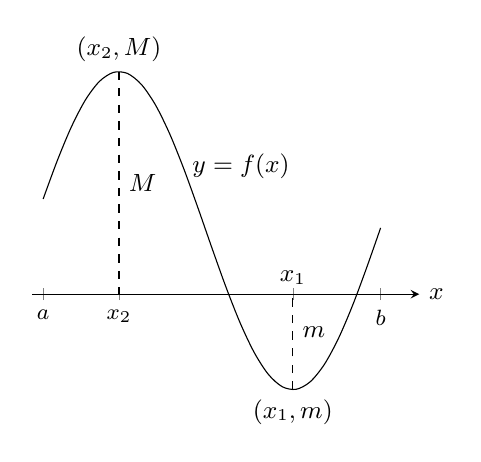
\begin{tikzpicture}[font=\small,declare function={f(\x)=0.4+sin(deg(\x));}]
\pgfmathsetmacro{\kA}{f(1.571)}
\pgfmathsetmacro{\kB}{f(4.713)}
\begin{axis}[clip=false,small,axis lines=middle,xlabel={$x$},xtick={0.2,1.571,4.713,6.3},xticklabels={$a$,$x_2$,,$b$},ytick={\empty},xmin=0,xmax=7,xlabel style={at={(current axis.right of origin)},anchor=west},y axis line style={draw=none}]
\addplot[domain=0.2:6.3,smooth]{f(x)}node[pos=0.4,right]{$y=f(x)$};
\draw(axis cs:1.571,\kA)node[above]{$(x_2,M)$} (axis cs:4.713,\kB)node[below]{$(x_1,m)$};
\draw[dashed](axis cs:1.571,\kA)--(axis cs:1.571,0)node[pos=0.5,right]{$M$};
\draw[dashed](axis cs:4.713,\kB)--(axis cs:4.713,0)node[pos=0.6,right]{$\abs{m}$}node[above]{$x_1$};
\end{axis}
\end{tikzpicture}
\caption{زیادہ سے زیادہ اور کم سے کم قیمتیں اندرونی نقطوں پر ہیں۔}
\end{subfigure}%
\begin{subfigure}{0.5\textwidth}
\centering
\begin{tikzpicture}[font=\small]
\begin{axis}[small,axis lines=middle,xlabel={$x$},xlabel style={at={(current axis.right of origin)},anchor=west},y axis line style={draw=none},xmin=-0.5,xmax=2.5,ymin=0,ymax=1.5,ytick={\empty},xtick={0.2,2},xticklabels={$a$,$b$}]
\draw(axis cs:0.2,1) to [out=-40,in=170] node[pos=0.5,above right]{$y=f(x)$}(axis cs:2,0.5);
\draw[dashed](axis cs:0.2,1)--(axis cs:0.2,0)node[pos=0.5,right]{$M$};
\draw[dashed](axis cs:2,0.5)--(axis cs:2,0)node[pos=0.6,right]{$m$};
\end{axis}
\end{tikzpicture}
\caption{زیادہ سے زیادہ اور کم سے کم آخری نقطوں پر ہے۔}
\end{subfigure}
\begin{subfigure}{0.5\textwidth}
\centering
\begin{tikzpicture}[font=\small,declare function={f(\x)=1+(\x-1)^2;}]
\pgfmathsetmacro{\kA}{f(1)}
\pgfmathsetmacro{\kB}{f(2)}
\begin{axis}[clip=false,small,axis lines=middle,xlabel={$x$},xtick={0.2,1,2},xticklabels={$a$,$x_1$,$b$},ytick={\empty},xmin=0,xmax=2.5,ymin=0,xlabel style={at={(current axis.right of origin)},anchor=west},y axis line style={draw=none}]
\addplot[domain=0.2:2,smooth]{f(x)}node[pos=0.15,above right]{$y=f(x)$};
\draw[dashed](axis cs:1,\kA)--(axis cs:1,0)node[pos=0.5,right]{$m$};
\draw[dashed](axis cs:2,\kB)--(axis cs:2,0)node[pos=0.6,right]{$M$};
\end{axis}
\end{tikzpicture}
\caption{کم سے کم اندرونی نقطہ جبکہ زیادہ سے زیادہ آخری نقطہ ہے۔}
\end{subfigure}%
\begin{subfigure}{0.5\textwidth}
\centering
\begin{tikzpicture}[font=\small,declare function={f(\x)=sin(deg(\x));}]
\pgfmathsetmacro{\kA}{f(0.2)}
\pgfmathsetmacro{\kB}{f(3.142/2)}
\begin{axis}[clip=false,small,axis lines=middle,xlabel={$x$},xtick={0.2,1.571,2.6},xticklabels={$a$,$x_2$,$b$},ytick={\empty},xmin=0,xmax=3,ymin=0,xlabel style={at={(current axis.right of origin)},anchor=west},y axis line style={draw=none}]
\addplot[domain=0.2:2.6,smooth]{f(x)}node[pos=0.15,below right]{$y=f(x)$};
\draw[dashed](axis cs:0.2,\kA)--(axis cs:0.2,0)node[pos=0.5,right]{$m$};
\draw[dashed](axis cs:1.571,\kB)--(axis cs:1.571,0)node[pos=0.6,right]{$M$};
\end{axis}
\end{tikzpicture}
\caption{زیادہ سے زیادہ اندرونی نقطہ جبکہ کم سے کم  آخری نقطہ پر ہے۔}
\end{subfigure}
\caption{زیادہ سے زیادہ اور کم سے کم نقطوں کے چند ممکنہ مقامات۔}
\label{شکل_استعمال_بلند_تر_کم_تر}
\end{figure}

\ابتدا{مثال}\شناخت{مثال_استعمال_انتہائی_سائن_کوسائن}
وقفہ \عددی{[-\pi/2,\pi/2]} پر تفاعل \عددی{f(x)=\cos x} ایک بار زیادہ سے زیادہ قیمت \عددی{1} اور دو بار کم سے کم  قیمت \عددی{0} اختیار کرتا ہے۔اسی وقفے پر  تفاعل \عددی{g(x)=\sin x} ایک بار زیادہ سے زیادہ  قیمت \عددی{1} اور ایک بار کم سے کم قیمت \عددی{-1} اختیار کرتا ہے (شکل \حوالہ{شکل_مثال_استعمال_انتہائی_سائن_کوسائن})۔ 
\begin{figure}
\centering
\begin{tikzpicture}
\begin{axis}[clip=false,small,axis lines=middle,xlabel={$x$},ylabel={$y$},ytick={-1,1},xtick={-1.571,1.571},xticklabels={$-\tfrac{\pi}{2}$,$\tfrac{\pi}{2}$},ymin=-1.2,ymax=1.5,xmin=-2,xmax=2]
\addplot[domain=-1.571:1.571]{cos(deg(x))}node[pos=0.25,above left]{$y=\cos x$};
\addplot[domain=-1.571:1.571]{sin(deg(x))}node[right]{$y=\sin x$};
\addplot[draw=none,mark=*] plot coordinates{(-1.571,0) (1.571,0) (-1.571,-1) (1.571,1) (0,1)};
\end{axis}
\end{tikzpicture}
\caption{ترسیم برائے مثال \حوالہ{مثال_استعمال_انتہائی_سائن_کوسائن}}
\label{شکل_مثال_استعمال_انتہائی_سائن_کوسائن}
\end{figure}
\انتہا{مثال}
%==============================

جیسا شکل \حوالہ{شکل_استعمال_بلند_تر_کم_تر_غیر_یقینی} اور شکل \حوالہ{شکل_استعمال_استمراری_ضروری_ورنہ} واضح کرتے ہیں مسئلہ \حوالہ{مسئلہ_استعمال_بلند_تر_کمتر} میں دائرہ کار کا بند ہونا اور تفاعل کا استمراری ہونا لازمی ہے۔ان کے بغیر مسئلے سے اخذ نتائج غلط ہو سکتے ہیں۔
\begin{figure}
\centering
\begin{minipage}{0.45\textwidth}
\centering
\begin{tikzpicture}[declare function={f(\x)=\x;}]
\begin{axis}[clip=false,small,axis lines=middle,xlabel={$x$},ylabel={$y$},xtick={1},ytick={1},xmin=-0.2,xmax=1.5,ymin=-0.2,ymax=1.5,ylabel style={at={(current axis.above origin)},anchor=south}]
\addplot[domain=0:1] {f(x)}node[pos=0.6,below right,align=center]{$y=x$\\  $0<x<1$};
\draw(axis cs:0,0)node[ocirc]{}node[pin=135:{\RL{کم سے کم قیمت موجود نہیں}}]{} (axis cs:1,1)node[ocirc]{}node[pin=135:{\RL{زیادہ سے زیادہ قیمت موجود نہیں}}]{};
\end{axis}
\end{tikzpicture}
\caption{کھلا وقفہ پر زیادہ سے زیادہ اور کم سے کم قیمتوں کا ہونا یقینی نہیں ہے۔}
\label{شکل_استعمال_بلند_تر_کم_تر_غیر_یقینی}
\end{minipage}\hfill
\begin{minipage}{0.45\textwidth}
\centering
\begin{tikzpicture}
\begin{axis}[clip=false,small,axis lines=middle,xmin=-1.25,xmax=1.5,ymin=-1.25,ymax=1.5]
\addplot[domain=-1:0]{x+1}node[pos=0.4,above left,align=center]{$y=x+1$\\  $-1\le x<0$};
\addplot[domain=0:1]{x-1}node[pos=0.6,below right,align=center]{$y=x-1$\\  $0<x\le 1$};
\draw(axis cs:-1,0)node[circ]{} (axis cs:0,1)node[ocirc]{}node[pin=0:{\RL{زیادہ سے زیادہ  قیمت موجود نہیں}}]{}  (axis cs:0,-1)node[ocirc]{}node[pin=-30:{\RL{کم سے کم قیمت موجود نہیں}}]{}  (axis cs:1,0)node[circ]{};
\end{axis}
\end{tikzpicture}
\caption{واحد ایک نقطہ عدم استمرار کی بنا زیادہ سے زیادہ اور کم سے کم قیمتیں غیر یقینی ہو سکتے ہیں۔}
\label{شکل_استعمال_استمراری_ضروری_ورنہ}
\end{minipage}
\end{figure} 

شکل \حوالہ{شکل_استعمال_استمراری_ضروری_ورنہ} میں تفاعل
\begin{align*}
f(x)=
\begin{cases}
x+1,&-1\le x<0\\ 
0,&x=0\\
x-1,&0<x\le 1
\end{cases}
\end{align*}
دکھایا گیا ہے جو وقفہ \عددی{[-1,1]} پر استمراری ہے ماسوائے واحد نقطہ \عددی{x=0}  پر، جس کی بنا تفاعل کا نا کوئی زیادہ سے زیادہ قیمت اور نا ہی اس کی کوئی کم سے کم قیمت پائی جاتی ہے۔

\جزوحصہء{مقامی بالمقابل مطلق (عالمگیر) انتہا}
شکل \حوالہ{شکل_استعمال_مقامی_مطلق_انتہا} میں تفاعل کے پانچ انتہا نقطے دکھائے گئے ہیں۔اس تفاعل کا کم سے کم نقطہ \عددی{a} پر ہے اگرچہ \عددی{e} پر بھی \عددی{x} کی مقامی قیمتوں کے لحاظ سے \عددی{f} کی قیمت کم ہے۔نقطہ \عددی{c} پر تفاعل کی مقامی زیادہ سے زیادہ قیمت پائی جاتی ہے جبکہ \عددی{d} پر اس کی مطلق زیادہ سے زیادہ قیمت پائی جاتی ہے۔
\begin{figure}
\centering
\begin{tikzpicture}
\draw[-latex](-0.25,0)--(4,0)node[right]{$x$};
\draw(0,0.5) to [out=45,in=180] (1.25,1.3) to [out=0,in=180] (2,1) to [out=0,in=180] (3,2) to [out=-45,in=170] (3.5,1.5);
\draw[dashed] (0,0.5)--(0,0)node[below]{$a$}  (1.25,1.3)--(1.25,0)node[below]{$c$}  (2,1)--(2,0)node[below]{$e$}  (3,2)--(3,0)node[below]{$d$}   (3.5,1.5)--(3.5,0)node[below]{$b$};
\draw(0.75,1.3)--(1.75,1.3)   (1.5,1)--(2.5,1);
\draw(0,0.5)node[left]{\RL{مطلق کم سے کم}};
\draw(1.25,1.3)node[above]{\RL{مقامی زیادہ سے زیادہ}};
\draw(2,1)node[below]{\RL{مقامی کم سے کم}};
\draw(3,2)node[above]{\RL{مطلق زیادہ سے زیادہ}};
\draw(3.5,1.5)node[right]{\RL{مقامی کم سے کم}};
\end{tikzpicture}
\caption{مقامی اور مطلق انتہا۔}
\label{شکل_استعمال_مقامی_مطلق_انتہا}
\end{figure}

\ابتدا{تعریف}\موٹا{مطلق انتہائی قیمتیں}\\
فرض کریں تفاعل \عددی{f} کا دائرہ کار \عددی{D} ہے۔نقطہ \عددی{c} پر تفاعل \عددی{f} کی مطلق زیادہ سے زیادہ قیمت  تب پائی جائے گی جب \عددی{D} میں تمام \عددی{x} کے لئے درج ذیل ہو
\begin{align*}
f(x)\le f(c)
\end{align*}
اور \عددی{D} میں \عددی{c} پر تب \عددی{f} کی مطلق کم سے کم قیمت  پائی جائے گی  جب \عددی{D} میں تمام \عددی{x} کے لئے درج ذیل ہو۔
\begin{align*}
f(x)\ge f(c)
\end{align*} 
\انتہا{تعریف}
%========================

مطلق زیادہ سے زیادہ  اور مطلق کم سے کم کو  مطلق \اصطلاح{انتہا}\فرہنگ{انتہا}\حاشیہب{extrema}\فرہنگ{extrema} کہتے ہیں۔انہیں \اصطلاح{عالمگیر}\فرہنگ{عالمگیر}\حاشیہب{global}\فرہنگ{global} انتہا بھی کہتے ہیں۔

ایک جیسے قاعدہ کے تفاعل کی انتہا قیمتیں مختلف ہو سکتی ہیں۔ انتہا قیمتیں دائرہ کار پر بھی منحصر ہوں گی۔

\ابتدا{مثال}\شناخت{مثال_استعمال_مطلق_قیمت_دائرہ_کار}
\begin{align*}
\begin{array}{cccr}
&\text{قاعدہ تفاعل}&  D\,\text{دائرہ کار}&\multicolumn{1}{c}{\text{مطلق انتہا}}\\
\hline
\text{(ا)}&y=x^2&(-\infty,\infty)& \text{مطلق زیادہ سے زیادہ نہیں ہے جبکہ \عددی{x=0} پر مطلق کم سے کم قیمت \عددی{0} ہے}\\
\text{(ب)}&y=x^2&[0,2]&\text{مطلق زیادہ سے زیادہ قیمت \عددی{x=2} پر \عددی{4} ہے جبکہ \عددی{x=0} پر مطلق کم سے کم قیمت \عددی{0} ہے}\\
\text{(ج)}&y=x^2&(0,2]&\text{مطلق زیادہ سے زیادہ قیمت \عددی{x=2} پر \عددی{4} ہے جبکہ مطلق کم سے کم قیمت موجود نہیں ہے}\\
\text{(د)}&y=x^2&(0,2)&\text{کوئی مطلق قیمت نہیں پایا جاتا ہے}
\end{array}
\end{align*}
شکل \حوالہ{شکل_مثال_استعمال_مطلق_قیمت_دائرہ_کار} دیکھیں۔
\begin{figure}
\centering
\begin{subfigure}{0.5\textwidth}
\centering
\begin{tikzpicture}
\begin{axis}[small,axis lines=middle,xlabel={$x$},ylabel={$y$},xtick={-2,2},ytick={\empty},xlabel style={at={(current axis.right of origin)},anchor=west},xmin=-2.5,xmax=2.5,ymin=-0.2]
\addplot[domain=-2.25:2.25]{x^2};
\draw(axis cs:0,0)node[circ]{};
\draw(axis cs:0,2)node[fill=white,align=center]{$y=x^2$\\  $D:(-\infty,\infty)$};
\end{axis}
\end{tikzpicture}
\caption{مطلق کم سے کم قیمت پائی جاتی ہے}
\end{subfigure}%
\begin{subfigure}{0.5\textwidth}
\centering
\begin{tikzpicture}
\begin{axis}[small,axis lines=middle,xlabel={$x$},ylabel={$y$},xtick={-2,2},ytick={\empty},xlabel style={at={(current axis.right of origin)},anchor=west},xmin=-2.5,xmax=2.5,ymin=-0.2]
\addplot[domain=-2.25:2.25]{x^2};
\draw(axis cs:0,0)node[circ]{}  (axis cs:2,4)node[circ]{};
\draw(axis cs:0,2)node[fill=white,align=center]{$y=x^2$\\  $D:[0,2]$};
\end{axis}
\end{tikzpicture}
\caption{مطلق کم سے کم اور زیادہ سے زیادہ قیمت پائی جاتی ہیں}
\end{subfigure}
\begin{subfigure}{0.5\textwidth}
\centering
\begin{tikzpicture}
\begin{axis}[small,axis lines=middle,xlabel={$x$},ylabel={$y$},xtick={-2,2},ytick={\empty},xlabel style={at={(current axis.right of origin)},anchor=west},xmin=-2.5,xmax=2.5,ymin=-0.2]
\addplot[domain=-2.25:2.25]{x^2};
\draw(axis cs:0,0)node[ocirc]{}  (axis cs:2,4)node[circ]{};
\draw(axis cs:0,2)node[fill=white,align=center]{$y=x^2$\\  $D:(0,2]$};
\end{axis}
\end{tikzpicture}
\caption{مطلق  زیادہ سے زیادہ قیمت پائی جاتی ہے}
\end{subfigure}%
\begin{subfigure}{0.5\textwidth}
\centering
\begin{tikzpicture}
\begin{axis}[small,axis lines=middle,xlabel={$x$},ylabel={$y$},xtick={-2,2},ytick={\empty},xlabel style={at={(current axis.right of origin)},anchor=west},xmin=-2.5,xmax=2.5,ymin=-0.2]
\addplot[domain=-2.25:2.25]{x^2};
\draw(axis cs:0,0)node[ocirc]{}  (axis cs:2,4)node[ocirc]{};
\draw(axis cs:0,2)node[fill=white,align=center]{$y=x^2$\\  $D:(0,2)$};
\end{axis}
\end{tikzpicture}
\caption{نا مطلق زیادہ سے زیادہ اور نا مطلق کم سے کم قیمت پائی جاتی ہے}
\end{subfigure}
\caption{مطلق قیمت اور دائرہ کار (مثال \حوالہ{مثال_استعمال_مطلق_قیمت_دائرہ_کار})۔}
\label{شکل_مثال_استعمال_مطلق_قیمت_دائرہ_کار}
\end{figure}
\انتہا{مثال}
%========================

\ابتدا{تعریف}\موٹا{مقامی انتہا قیمت}\\
تفاعل \عددی{f} کا کھلے دائرہ کار \عددی{D} میں اندرونی نقطہ \عددی{c} پر اس صورت مقامی زیادہ سے زیادہ قیمت پائی جائے گی جب \عددی{D} میں کسی بھی کھلا وقفہ جس میں \عددی{c} پایا جاتا ہو میں تمام \عددی{x} کے لئے
\begin{align*}
f(x)\le f(c)
\end{align*}
ہو جبکہ (انہیں شرائط کے ساتھ) درج ذیل صورت میں  اندرونی نقطہ \عددی{c} پر مقامی زیادہ سے زیادہ قیمت پائی جائے گی۔
\begin{align*}
f(x)\ge f(c)
\end{align*} 
\انتہا{تعریف}
%===========================

ہم مقامی انتہا کی تعریف کو وقفہ کے آخری سروں تک وسعت دے سکتے ہیں۔یوں آخری سر \عددی{c} پر مقامی انتہا سے مراد نصف کھلا وقفہ میں موزوں عدم مساوات کا مطمئن ہونا ہے۔ شکل \حوالہ{شکل_استعمال_مقامی_مطلق_انتہا} میں تفاعل \عددی{f} کا \عددی{c} اور \عددی{d} پر مقامی زیادہ سے زیادہ قیمت جبکہ  \عددی{a}، \عددی{e} اور \عددی{b} پر اس کی مقامی کم سے کم قیمت پائی جاتی ہیں۔

مطلق زیادہ سے زیادہ قیمت بھی مقامی زیادہ سے زیادہ قیمت ہو گی۔مطلق زیادہ سے زیادہ قیمت اپنی پڑوس میں بھی زیادہ سے زیادہ قیمت ہو گی۔یوں تمام مقامی زیادہ سے زیادہ قیمتوں کی جدول میں مطلق زیادہ سے زیادہ قیمت (اگر موجود ہو) بھی پائی جائے گی۔ اسی طرح تمام مقامی کم سے کم قیمتوں کی جدول میں مطلق کم سے کم قیمت (اگر موجود ہو) بھی پائی جائے گی۔

\جزوحصہء{انتہا کا حصول}
جیسا درج ذیل مسئلہ سمجھاتا ہے تفاعل کے  انتہا کی حصول کے لئے صرف چند قیمتوں کی تحقیق ضروری ہو گی۔

\ابتدا{مسئلہ}\شناخت{مسئلہ_استعمال_یک_درجی_تفرق_انتہا}\موٹا{یک درجی مسئلہ برائے مقامی انتہا}
فرض کریں  تفاعل \عددی{f} کے دائرہ کار کی اندرونی نقطہ \عددی{c} پر \عددی{f} کی کم سے کم یا زیادہ سے زیادہ قیمت پائی جاتی ہو اور \عددی{c} پر \عددی{f'} معین ہو تب درج ذیل ہو گا۔
\begin{align*}
f'(c)=0
\end{align*} 
\انتہا{مسئلہ}
%=====================
\ابتدا{ثبوت}
یہ دکھانے کی خاطر کہ مقامی انتہا پر \عددی{f'(c)} کی قیمت صفر ہو گی ہم  دکھاتے ہیں کہ \عددی{f'(c)} مثبت نہیں ہو سکتا ہے اور  کہ \عددی{f'(c)} منفی نہیں ہو سکتا ہے۔صفر وہ  واحد عدد ہے جو نا مثبت اور نا منفی ہے لہٰذا \عددی{f'(c)} صفر ہو گا۔   

فرض کریں کہ \عددی{c} پر \عددی{f} کی مقامی زیادہ سے زیادہ قیمت پائی جاتی ہے (شکل \حوالہ{شکل_مسئلہ_استعمال_یک_درجی_تفرق_انتہا})۔ یوں \عددی{c} کے قریبی پڑوس میں تمام \عددی{x} پر \عددی{f(x)-f(c)\le 0} ہو گا۔چونکہ \عددی{c} اندرونی نقطہ ہے لہٰذا \عددی{f'(c)} کی تعریف درج ذیل دو طرفہ حد ہو گی۔
\begin{align*}
\lim_{x\to c}\frac{f(x)-f(c)}{x-c}
\end{align*}
اس کا مطلب ہے کہ \عددی{x=c} پر دائیں ہاتھ حد اور بائیں ہاتھ حد دونوں موجود اور \عددی{f'(c)} کے برابر ہیں۔ان حد پر علیحدہ علیحدہ غور کرتے ہیں۔چونکہ \عددی{c} کے دائیں جانب \عددی{x-c>0} اور \عددی{f(x)\le f(c)} ہیں لہٰذا
\begin{align}\label{مساوات_استعمال_یک_درجی_تفرق_الف}
f'(c)=\lim_{x\to c^+}\frac{f(x)-f(c)}{x-c}\le 0
\end{align}
ہو گا۔اسی طرح \عددی{c} کے بائیں جانب \عددی{x-c<0} اور \عددی{f(x)\le f(c)} ہیں لہٰذا
\begin{align}\label{مساوات_استعمال_یک_درجی_تفرق_ب}
f'(c)=\lim_{x\to c^-}\frac{f(x)-f(c)}{x-c}\ge 0
\end{align}
ہو گا۔مساوات \حوالہ{مساوات_استعمال_یک_درجی_تفرق_الف} اور مساوات \حوالہ{مساوات_استعمال_یک_درجی_تفرق_ب} کو ملا کر \عددی{f'(c)=0} ملتا ہے۔

یوں مقامی زیادہ سے زیادہ قیمت کے لئے مسئلہ ثابت ہوا۔مقامی کم سے کم قیمت کے لئے مسئلہ ثابت کرنے کے لئے \عددی{f(x)\ge f(c)} استعمال کرنا ہو گا جس سے مساوات \حوالہ{مساوات_استعمال_یک_درجی_تفرق_الف} اور مساوات \حوالہ{مساوات_استعمال_یک_درجی_تفرق_ب} کی عدم مساوات الٹ ہو جاتی ہیں۔
\begin{figure}
\centering
\begin{tikzpicture}[font=\small,y=2cm,x=2cm,declare function={f(\x)=1.5-\x*\x;}]
\pgfmathsetmacro{\kA}{f(0.2)}
\pgfmathsetmacro{\kB}{f(0.4)}
\pgfmathsetmacro{\kC}{f(0.6)}
\draw[-latex] (-1.5,0)--(1.5,0)node[right]{$x$};
\draw[name path=kC,domain=-1:1] plot ({\x},{1.5-\x*\x})node[right]{$y=f(x)$};
\draw(-1,1.5)--(1,1.5);
\draw[shorten <=-0.5cm, shorten >=-0.5cm](0,1.5)--(0.2,\kA);
\draw[shorten <=-0.5cm, shorten >=-0.5cm](0,1.5)--(0.4,\kB);
\draw[shorten <=-0.5cm, shorten >=-0.5cm](0,1.5)--(0.6,\kC);
\draw[shorten <=-0.5cm, shorten >=-0.5cm](0,1.5)--(-0.2,\kA);
\draw[shorten <=-0.5cm, shorten >=-0.5cm](0,1.5)--(-0.4,\kB);
\draw[shorten <=-0.5cm, shorten >=-0.5cm](0,1.5)--(-0.6,\kC);
\draw[dashed] (-0.6,\kC)--(-0.6,0)node[below]{$x$};
\draw[dashed] (0,1.5)--(0,0)node[below]{$c$};
\draw[dashed] (0.6,\kC)--(0.6,0)node[below]{$x$};
\draw(0,1.5)node[pin=90:{\RL{مقامی انتہا}}]{};
\draw(-0.5,0.5)node[fill=white,align=center]{\RL{غیر منفی}\\ \RL{ڈھلوان سیکنٹ}};
\draw(0.5,0.5)node[fill=white,align=center]{\RL{غیر مثبت}\\ \RL{ڈھلوان سیکنٹ}};
\end{tikzpicture}
\caption{اندرونی نقطہ پر مقامی انتہا پر ڈھلوان صفر ہو گی (مسئلہ \حوالہ{مسئلہ_استعمال_یک_درجی_تفرق_انتہا})۔}
\label{شکل_مسئلہ_استعمال_یک_درجی_تفرق_انتہا}
\end{figure}
\انتہا{ثبوت}
%======================

مسئلہ \حوالہ{مسئلہ_استعمال_یک_درجی_تفرق_انتہا} کہتا ہے کہ اندرونی انتہا پر اگر تفرق معین ہو تب \عددی{f'(c)=0} ہو گا۔ یوں تفاعل کی انتہا (مقامی یا عالمگیر) صرف درج ذیل نقطوں پر ہو سکتی ہیں۔
\begin{enumerate}[1.]
\item
اندرونی نقطہ جہاں \عددی{f'=0} ہو۔\\
\item
اندرونی نقطہ جہاں \عددی{f'} غیر معین ہو۔\\
\item
\عددی{f} کے دائرہ کار کے آخری سروں پر۔
\end{enumerate}

درج ذیل تعریف ان نتائج کو مختصراً پیش کرنے میں مدد کرتی ہے۔

\ابتدا{تعریف}
تفاعل \عددی{f} کے دائرہ کار میں ایسا اندرونی نقطہ جہاں \عددی{f'} غیر معین یا صفر ہو کو \اصطلاح{نقطہ فاصل}\فرہنگ{نقطہ فاصل}\حاشیہب{critical point}\فرہنگ{critical point} کہتے ہیں۔ 
\انتہا{تعریف}

\موٹا{خلاصہ}\\
تفاعل کی انتہا قیمتیں صرف تفاعل کی دائرہ کار میں نقطہ فاصل اور آخری نقطوں  پر پائی جا سکتی ہیں۔ 

عموماً بند دائرہ کار پر تفاعل  کی انتہا  مطلوب ہو گی۔ مسئلہ \حوالہ{مسئلہ_استعمال_بلند_تر_کمتر} ہمیں یقین دلاتا ہے کہ ایسی قیمتیں موجود ہوں گی؛  مسئلہ \حوالہ{مسئلہ_استعمال_یک_درجی_تفرق_انتہا} کہتا ہے کہ یہ صرف آخری نقطوں پر اور نقطہ فاصل پر پائی جائیں گی۔اس قسم کے نقطے عموماً چند ہوں گے جن کی فہرست تیار کر کے دیکھا جا سکتا ہے کہ آیا نقطہ پر زیادہ سے زیادہ یا کم سے کم قیمت پائی جاتی ہے۔

\ابتدا{مثال}
دائرہ کار \عددی{[-2,1]} پر تفاعل \عددی{f(x)=x^2} کی مطلق زیادہ سے زیادہ اور مطلق کم سے کم قیمتیں تلاش کریں۔\\
حل:\quad
تفاعل پورے دائرہ کار پر قابل تفرق ہے لہٰذا واحد نقطہ فاصل \عددی{f'(x)=2x=0} یعنی \عددی{x=0} پر ہو گا۔ہمیں تفاعل کی قیمتیں نقطہ فاصل \عددی{x=0} اور آخری نقطوں \عددی{x=-2} اور \عددی{x=1} پر دیکھنی ہوں گی۔
\begin{align*}
f(0)&=0&&\text{نقطہ فاصل پر قیمت}\\
f(-2)&=4&&\text{آخری نقطہ پر قیمت}\\
f(1)&=1&&\text{آخری نقطہ پر قیمت}
\end{align*}
تفاعل کی مطلق زیادہ سے زیادہ قیمت \عددی{4} ہے جو نقطہ \عددی{x=-2} پر پائی جاتی ہے جبکہ اس کی مطلق کم سے کم قیمت \عددی{0} ہے جو نقطہ \عددی{x=0} پر پائی جاتی ہے۔
\انتہا{مثال}
%===================
\ابتدا{سوال}\شناخت{مثال_استعمال_مطلق_انتہا_الف}
دائرہ کار \عددی{[-2,1]} پر تفاعل \عددی{g(t)=8t-t^4} کی مطلق زیادہ سے زیادہ اور مطلق کم سے کم قیمت تلاش کریں۔\\
حل:\quad تفرق پورے دائرہ کار پر قابل تفرق ہے لہٰذا نقطہ فاصل صرف وہاں ہو گا جہاں \عددی{g'(t)=0} ہو۔ اس مساوات کو حل کرتے ہوئے
\begin{align*}
g'(t)&=8-4t^3=0\\
t^3&=2\\
t&=2^{1/3}
\end{align*}
ملتا ہے جو دائرہ کار کے اندر نہیں ہے۔یوں تفاعل کے مقامی انتہا قیمتیں آخری نقطوں پر پائی جائیں گی: (شکل \حوالہ{شکل_مثال_استعمال_مطلق_انتہا_الف})
\begin{align*}
g(-2)&=-32&&\text{مطلق کم سے کم قیمت}\\
g(1)&=7&&\text{مطلق زیادہ سے زیادہ قیمت}
\end{align*}
%
\begin{figure}
\centering
\begin{minipage}{0.45\textwidth}
\centering
\begin{tikzpicture}[font=\small]
\begin{axis}[clip=false,small,axis lines=middle,xlabel={$t$},ylabel={$y$},xtick={-2,1},ytick={-32,7},xmin=-2.5,xmax=1.5,ymin=-35,ymax=9]
\addplot[domain=-2:1]{8*x-x^4}node[pos=0.25,right]{$g(t)=8t-t^4$};
\draw(axis cs:1,7)node[circ]{}node[above]{$(1,7)$}  (axis cs:-2,-32)node[circ]{}node[below]{$(-2,-32)$};
\end{axis}
\end{tikzpicture}
\caption{ترسیم برائے مثال \حوالہ{مثال_استعمال_مطلق_انتہا_الف}}
\label{شکل_مثال_استعمال_مطلق_انتہا_الف}
\end{minipage}\hfill
\begin{minipage}{0.45\textwidth}
\centering
\begin{tikzpicture}[font=\small]
\begin{axis}[clip=false,small,axis lines=middle,xlabel={$x$},ylabel={$y$},xtick={-2,-1,1,2,3},ytick={1,2},xmin=-3,xmax=4.5]
\addplot[domain=-0.5:0]{(x^2)^(1/3)};
\addplot[domain=0:0.5]{(x^2)^(1/3)};
\addplot[domain=-2:-0.5]{(x^2)^(1/3)};
\addplot[domain=0.5:3]{(x^2)^(1/3)}node[pos=0.25,right]{$y=x^{2/3}$};
\draw(axis cs:-2,1.587)node[circ]{}node[above]{\RL{مقامی زیادہ سے زیادہ}}  (axis cs:3,2.08)node[circ]{}node[above]{\RL{مطلق اور مقامی زیادہ سے زیادہ}};
\end{axis}
\end{tikzpicture}
\caption{ترسیم برائے مثال \حوالہ{مثال_استعمال_مطلق_انتہا_ب}}
\label{شکل_مثال_استعمال_مطلق_انتہا_ب}
\end{minipage}
\end{figure}
\انتہا{سوال}
%======================
\ابتدا{سوال}\شناخت{مثال_استعمال_مطلق_انتہا_ب}
تفاعل \عددی{h(x)=x^{2/3}} کی  \عددی{[-2,-3]} پر مطلق انتہا تلاش کریں۔\\
حل:\quad
یک درجی تفرق
\begin{align*}
h'(x)=\frac{2}{3}x^{-1/3}=\frac{2}{3x^{1/3}}
\end{align*}
کا صفر نہیں پایا جاتا ہے البتہ \عددی{x=0} پر یہ غیر معین ہے۔اس نقطہ پر اور آخری نقطوں \عددی{x=-2} اور \عددی{x=3} پر تفاعل کی قیمتیں درج ذیل ہیں۔
\begin{align*}
h(0)&=0\\
h(-2)&=(-2)^{2/3}=4^{1/3}\\
h(3)&=(3)^{2/3}=9^{1/3}
\end{align*}
مطلق زیادہ سے زیادہ قیمت \عددی{9^{1/3}} ہے جو نقطہ \عددی{x=3} پر پائی جاتی ہے جبکہ مطلق کم سے کم قیمت \عددی{0} ہے جو نقطہ \عددی{x=0} پر پائی جاتی ہے  (شکل \حوالہ{شکل_مثال_استعمال_مطلق_انتہا_ب})۔
\انتہا{سوال}
%=====================

اگرچہ تفاعل کی انتہا صرف نقطہ فاصل اور آخری نقطوں پر پائی جا سکتی ہیں، ضروری نہیں ہے کہ ہر نقطہ فاصل یا ہر آخری نقطہ  پر انتہا قیمت پائی جاتی ہو۔ شکل \حوالہ{شکل_مثال_استعمال_نقطہ_فاصل_نہیں_الف} اور شکل \حوالہ{شکل_مثال_استعمال_نقطہ_فاصل_نہیں_ب} اندرونی نقطوں کے لئے اس حقیقت کی وضاحت کرتی ہے۔
\begin{figure}
\centering
\begin{minipage}{0.45\textwidth}
\centering
\begin{tikzpicture}
\begin{axis}[small,axis lines=middle,xlabel={$x$},ylabel={$y$},xtick={-1,1},ytick={-1,1}]
\addplot[domain=0:0.01]{x^(1/3)};
\addplot[domain=0:0.01]({-x},{-x^(1/3)});
\addplot[domain=0.01:0.5]{x^(1/3)};
\addplot[domain=0.01:0.5]({-x},{-x^(1/3)});
\addplot[domain=0.5:2]{x^(1/3)}node[pos=0.5,below]{$y=x^{1/3}$};
\addplot[domain=0.5:2]({-x},{-x^(1/3)});
\end{axis}
\end{tikzpicture}
\caption{نقطہ فاصل \عددی{x=0} پر انتہائی قیمت نہیں پائی جاتی ہے۔}
\label{شکل_مثال_استعمال_نقطہ_فاصل_نہیں_الف}
\end{minipage}\hfill
\begin{minipage}{0.45\textwidth}
\centering
\begin{tikzpicture}
\begin{axis}[small,axis lines=middle,xlabel={$x$},ylabel={$y$},xtick={-1,1},ytick={-1,1},xmin=-1.5,xmax=1.5,ymin=-1.5,ymax=1.5]
\addplot[domain=-1:1]{x^3}node[pos=0.9,left]{$y=x^3$};
\end{axis}
\end{tikzpicture}
\caption{
\عددی{x=0} پر \عددی{y=x^3} کا کوئی انتہا نہیں پایا جاتا ہے اگرچہ اس نقطے پر \عددی{y'=3x^2=0} ہے۔
}
\label{شکل_مثال_استعمال_نقطہ_فاصل_نہیں_ب}
\end{minipage}
\end{figure} 

\حصہء{سوالات}
\موٹا{ترسیم سے انتہائی نقطوں کا حصول}\\
کیا سوال \حوالہ{سوال_استعمال_ترسیم_سے_مطلق_الف} تا سوال \حوالہ{سوال_استعمال_ترسیم_سے_مطلق_الف} میں \عددی{[a,b]} کے بیچ تفاعل کے مطلق انتہائی قیمتیں پائی جاتی ہیں؟ سمجھائیں کہ آپ کے جواب اور مسئلہ \حوالہ{مسئلہ_استعمال_بلند_تر_کمتر} میں کس طرح تضاد نہیں پایا جاتا ہے۔

\ابتدا{سوال}\شناخت{سوال_استعمال_ترسیم_سے_مطلق_الف}

\انتہا{سوال}
%===================
\موٹا{بند وقفہ پر مطلق انتہا}

سوال \حوالہ{سوال_استعمال_مطلق_قیمتیں_تلاش_الف} تا سوال \حوالہ{سوال_استعمال_مطلق_قیمتیں_تلاش_ب} میں دیے گئے وقفے پر تفاعل کی مطلق انتہائی قیمتیں تلاش کریں۔تفاعل کو ترسیم کرتے ہوئے انتہائی نقطوں کی نشاندہی کریں۔

\ابتدا{سوال}\شناخت{سوال_استعمال_مطلق_قیمتیں_تلاش_الف}
$f(x)=\frac{2}{3}x-5,\quad -2\le x\le 3$
\انتہا{سوال}
%======================
\ابتدا{سوال}
$f(x)=-x-4,\quad -4\le x\le 1$
\انتہا{سوال}
%======================
\ابتدا{سوال}
$f(x)=x^2-1,\quad -1\le x\le 2$
\انتہا{سوال}
%======================
\ابتدا{سوال}
$f(x)=4-x^2,\quad -3\le x\le 1$
\انتہا{سوال}
%======================
\ابتدا{سوال}
$F(x)=-\tfrac{1}{x^2},\quad 0.5\le x\le 2$
\انتہا{سوال}
%======================
\ابتدا{سوال}
$F(x)=-\tfrac{1}{x},\quad -2\le x\le -1$
\انتہا{سوال}
%======================
\ابتدا{سوال}
$h(x)=\sqrt[3]{x},\quad -1\le x\le 8$
\انتہا{سوال}
%======================
\ابتدا{سوال}
$h(x)=-3x^{2/3},\quad -1\le x\le 1$
\انتہا{سوال}
%======================
\ابتدا{سوال}
$g(x)=\sqrt{4-x^2},\quad -2\le x\le 1$
\انتہا{سوال}
%======================
\ابتدا{سوال}
$g(x)=-\sqrt{5-x^2},\quad -\sqrt{5}\le x\le 0$
\انتہا{سوال}
%======================
\ابتدا{سوال}
$f(\theta)=\sin\theta,\quad -\tfrac{\pi}{2}\le \theta \le \tfrac{5\pi}{6}$
\انتہا{سوال}
%======================
\ابتدا{سوال}
$f(x)=\tan\theta,\quad -\tfrac{\pi}{3}\le \theta\le \tfrac{\pi}{4}$
\انتہا{سوال}
%======================
\ابتدا{سوال}
$g(x)=\csc x,\quad -\tfrac{\pi}{3}\le x \le \tfrac{2\pi}{3}$
\انتہا{سوال}
%======================
\ابتدا{سوال}
$g(x)=\sec x,\quad -\tfrac{\pi}{3}\le x\le \tfrac{\pi}{6}$
\انتہا{سوال}
%======================
\ابتدا{سوال}
$f(t)=2-\abs{t},\quad -1\le t\le 3$
\انتہا{سوال}
%======================
\ابتدا{سوال}\شناخت{سوال_استعمال_مطلق_قیمتیں_تلاش_ب}
$f(t)=\abs{t-5},\quad -4\le t\le 7$
\انتہا{سوال}
%======================
سوال \حوالہ{سوال_استعمال_مطلق_تلاش_الف} تا سوال \حوالہ{سوال_استعمال_مطلق_تلاش_ب} میں تفاعل کی مطلق کم سے کم اور مطلق زیادہ سے زیادہ قیمتیں تلاش کریں۔یہ قیمتیں کن نقطوں پر پائی جاتی ہیں؟

\ابتدا{سوال}\شناخت{سوال_استعمال_مطلق_تلاش_الف}
$f(x)=x^{4/3},\quad -1\le x\le 8$
\انتہا{سوال}
%===================
\ابتدا{سوال}
$f(x)=x^{5/3},\quad -1\le x\le 8$
\انتہا{سوال}
%===================
\ابتدا{سوال}
$g(\theta)=\theta^{3/5},\quad -32\le \theta \le 1$
\انتہا{سوال}
%===================
\ابتدا{سوال}\شناخت{سوال_استعمال_مطلق_تلاش_ب}
$h(\theta)=3\theta^{2/3},\quad -27\le \theta\le 8$
\انتہا{سوال}
%===================
\موٹا{دائرہ کار میں مقامی انتہا}

سوال \حوالہ{سوال_استعمال_مقامی_تلاش_الف} تا سوال \حوالہ{سوال_استعمال_مقامی_تلاش_الف} میں دی گئے دائرہ کار پر مقامی زیادہ سے زیادہ یا کم سے کم قیمت تلاش کریں۔یہ قیمتیں کن نقطوں پر پائی جاتی ہیں؟ ان میں سے کون سی مطلق انتہائی قیمتیں ہیں؟ 

\ابتدا{سوال}\شناخت{سوال_استعمال_مقامی_تلاش_الف}
\begin{multicols}{2}
\begin{enumerate}[a.]
\item
$f(x)=x^2-4,\quad -2\le x\le 2$
\item
$g(x)=x^2-4,\quad -2\le x<2$
\item
$h(x)=x^2-4,\quad -2<x<2$
\item
$k(x)=x^2-4,\quad -2\le x<\infty$
\item
$l(x)=x^2-4,\quad 0<x<\infty$
\end{enumerate}
\end{multicols}
\انتہا{سوال}
%========================
\ابتدا{سوال}
\begin{multicols}{2}
\begin{enumerate}[a.]
\item
$f(x)=2-2x^2,\quad -1\le x\le 1$
\item
$g(x)=2-2x^2,\quad -1<x\le 1$
\item
$h(x)=2-2x^2,\quad -1<x<1$
\item
$k(x)=2-2x^2,\quad -\infty<x\le 1$
\item
$l(x)=2-2x^2,\quad -\infty<x<0$
\end{enumerate}
\end{multicols}
\انتہا{سوال}
%========================
\موٹا{نظریہ اور مثالیں}

\ابتدا{سوال}
اگرچہ \عددی{x=0} پر \عددی{f(x)=\abs{x}} نا قابل تفرق ہے نقطہ \عددی{x=0}  پر \عددی{f} کی مطلق کم سے کم قیمت پائی جاتی ہے۔کیا یہ مسئلہ \حوالہ{مسئلہ_استعمال_یک_درجی_تفرق_انتہا} کے متضاد ہے؟ اپنے جواب کی وجہ پیش کریں۔
\انتہا{سوال}
%=========================== 
\ابتدا{سوال}
اگر تفاعل کے دائرہ کار کا آخری نقطہ \عددی{c} ہو تب مسئلہ \حوالہ{مسئلہ_استعمال_یک_درجی_تفرق_انتہا} کیوں نا قابل استعمال ہو گا؟
\انتہا{سوال}
%========================
\ابتدا{سوال}
اگر جفت تفاعل \عددی{f(x)} کی مقامی زیادہ سے زیادہ قیمت \عددی{x=c} پر پائی جاتی ہو تب \عددی{x=-c} پر اس کی قیمت کے بارے میں کیا کہنا ممکن ہو گا؟ اپنے جواب کی وجہ پیش کریں۔ 
\انتہا{سوال}
%==========================
\ابتدا{سوال}
اگر طاق تفاعل \عددی{g(x)} کی مقامی کم سے کم  قیمت \عددی{x=c} پر پائی جاتی ہو تب کیا  \عددی{x=-c} پر اس کی قیمت کے بارے میں کچھ کہنا ممکن ہو گا؟ اپنے جواب کی وجہ پیش کریں۔ 
\انتہا{سوال}
%==============================
\ابتدا{سوال}
ہم جانتے ہیں کہ نقطہ فاصل اور آخری نقطوں پر تفاعل \عددی{f(x)} کی قیمتوں کی جانچ پڑتال سے تفاعل کی انتہائی قیمتیں حاصل کی جا سکتی ہیں۔ کوئی بھی نقطہ فاصل یا آخری نقطہ نہ ہونا کی صورت میں کیا ہو گا؟ کیا ایسے تفاعل حقیقت میں پائے جاتے ہیں۔ اپنے جواب کی وجہ پیش کریں۔
\انتہا{سوال}
%================================
\ابتدا{سوال}
وقفہ \عددی{[0,1]} پر ایسا معین تفاعل پیش کریں جس کا \عددی{x=0} پر نا کوئی مقامی زیادہ سے زیادہ قیمت اور نا ہی مقامی کم سے کم قیمت پائی جاتی ہو۔
\انتہا{سوال}
%===============================
\موٹا{کمپیوٹر کا استعمال}\\
سوال \حوالہ{سوال_استعمال_کمپیوٹر_انتہائی_الف} تا سوال \حوالہ{سوال_استعمال_کمپیوٹر_انتہائی_ب} میں درج ذیل اقدام سے دیے گئے بند وقفہ میں تفاعل کی انتہائی قیمتیں تلاش کریں۔
\begin{enumerate}[a.]
\item
وقفہ  پر تفاعل تقسیم کرتے ہوئے اس کا رویہ دیکھیں۔
\item
 وہ اندرونی نقطے تلاش کریں جہاں \عددی{f'=0} ہو۔ بعض اوقات \عددی{f'} ترسیم  کرنا مددگار ثابت ہو گا۔
\item
وہ اندرونی نقطے تلاش کریں جہاں \عددی{f'} غیر موجود ہے۔
\item
جزو (ب) اور (ج) میں حاصل تمام نقطوں کے علاوہ دائرہ کار کے آخری نقطوں پر تفاعل کی قیمتیں حاصل کریں۔
\item
وقفہ پر تفاعل کی مطلق انتہائی قیمتیں اور جن نقطوں پر یہ قیمتیں پائی جاتی ہوں تلاش کریں۔ 

\end{enumerate}

\ابتدا{سوال}\شناخت{سوال_استعمال_کمپیوٹر_انتہائی_الف}
$f(x)=x^4-8x62+4x+2,\quad [-\tfrac{20}{25},\tfrac{64}{25}]$
\انتہا{سوال}
%======================
\ابتدا{سوال}
$f(x)=-x^4+4x^3-4x+1,\quad [-\tfrac{3}{4},3]$
\انتہا{سوال}
%=======================
\ابتدا{سوال}
$f(x)=x^{2/3}(3-x),\quad [-2,2]$
\انتہا{سوال}
%=======================
\ابتدا{سوال}
$f(x)=2+2x-3x^{2/3},\quad [-1,\tfrac{10}{3}]$
\انتہا{سوال}
%=======================
\ابتدا{سوال}
$f(x)=\sqrt{x}+\cos x,\quad [0,2\pi]$
\انتہا{سوال}
%=========================
\ابتدا{سوال}\شناخت{سوال_استعمال_کمپیوٹر_انتہائی_ب}
$f(x)=x^{3/4}-\sin x+\tfrac{1}{2},\quad [0,2\pi]$
\انتہا{سوال}
%=========================

\حصہ{مسئلہ اوسط قیمت}
ہم جانتے ہیں کہ سطح زمین کے قریب  ساکن حال (لمحہ \عددی{t=0}) سے گرتا ہوا  جسم ابتدائی \عددی{t} سیکنڈوں میں \عددی{s=4.9t^2\,\si{\meter}}  کا فاصل طے کرے گا۔اس معلومات کو استعمال کرتے ہوئے ہم کہہ سکتے ہیں کہ لمحہ \عددی{t} پر  اس جسم کی سمتی رفتار \عددی{v=\tfrac{\dif s}{\dif t}=\SI{9.8}{\meter\per\second}} اور اسراع
 \عددی{a=\tfrac{\dif^{\,2} s}{\dif t^2}=\SI{9.8}{\meter\per\second\squared}} ہو گی۔ اب فرض کریں کہ ہمیں جسم کی اسراع معلوم ہے۔ کیا ہم الٹ چلتے ہوئے اس کی سمتی رفتار اور ہٹاو تلاش کر سکتے ہیں؟

ہم حقیقت میں جاننا چاہتے ہیں کہ دیا گیا تفرق کس تفاعل کا ہو گا۔ زیادہ عمومی سوال یہ ہو گا کہ کس قسم کے تفاعل کا تفرق مخصوص قسم کا ہو گا۔ کس تفاعل کا تفرق مثبت ہو گا، یا منفی ہو گا، یا ہر نقطے پر صفر ہو گا؟ ان سوالات کے جوابات کو مسئلہ اوسط قیمت سے اخذ نتیجہ صریح  کی مدد سے حاصل کیا جا سکتا ہے۔

\جزوحصہء{مسئلہ رول}
جن دو نقطوں پر تفاعل \عددی{f(x)} محور \عددی{x} کو قطع  کرتا ہے اگر ان کے بیچ تفاعل قابل تفرق ہو تب \عددی{f(x)} کی  ترسیم کی جیومیٹری کو دیکھ کر ایسا معلوم ہوتا ہے کہ ان نقطوں کے بیچ کم سے کم ایک ایسا نقطہ ضرور پایا جائے گا جس پر تفاعل کا مماس افقی ہو۔ \ترچھا{مشل رول} \عددی{(1652-1719)} کا \عددی{300} سال پرانا \اصطلاح{مسئلہ رول} ہمیں یقین دہانی کراتا ہے کہ حقیقتاً ایسا ہی ہو گا۔

\ابتدا{مسئلہ}\شناخت{مسئلہ_استعمال_مسئلہ_رول}\موٹا{مسئلہ رول}\فرہنگ{مسئلہ!رول}\حاشیہب{Rolle's theorem}\فرہنگ{theorem!Rolle's}\\
فرض کریں بند وقفہ \عددی{[a,b]} کے ہر نقطہ پر تفاعل \عددی{y=f(x)} استمراری ہے اور وقفہ کی اندرون \عددی{(a,b)} کے ہر نقطہ پر تفاعل قابل تفرق ہے۔ اگر
\begin{align*}
f(a)=f(b)=0
\end{align*}
تب \عددی{(a,b)} میں کم سے کم ایسا ایک نقطہ \عددی{c} ہو گا جس پر درج ذیل ہو گا۔
\begin{align*}
f'(c)=0
\end{align*}
\انتہا{مسئلہ}
%======================
\ابتدا{ثبوت}
چونکہ \عددی{f} استمراری ہے لہٰذا \عددی{[a,b]} پر \عددی{f} کے مطلق زیادہ سے زیادہ اور مطلق کم سے کم قیمتیں ہوں گی۔یہ صرف درج ذیل نقطوں پر پائی جائیں گی۔
\begin{enumerate}[1.]
\item
ان اندرونی نقطوں پر جہاں \عددی{f'} ہو۔
\item
ان اندرونی نقطوں پر جہاں \عددی{f'} غیر معین ہو۔
\item
تفاعل کے دائرہ کار کی آخری نقطوں پر جو موجودہ صورت میں \عددی{a} اور \عددی{b} ہیں۔
\end{enumerate}
قیاس کے تحت ہر اندرونی نقطے پر \عددی{f} کا تفرق پایا جاتا ہے.یوں جزو (2) خارج ہوتا ہے۔

اگر وقفہ کے اندرونی نقطہ \عددی{c} پر تفاعل کی زیادہ سے زیادہ یا کم سے کم قیمت پائی جاتی ہو تب مسئلہ \حوالہ{مسئلہ_استعمال_یک_درجی_تفرق_انتہا} کے تحت \عددی{f'(c)=0} ہو گا جس سے مسئلہ رول کا نقطہ حاصل ہوتا ہے۔

اگر زیادہ سے زیادہ قیمت اور کم سے کم قیمت دونوں \عددی{a} یا \عددی{b} پر پائے جاتے ہوں تب \عددی{f} مستقل ہو گا۔یوں \عددی{f'=0} ہو گا لہٰذا وقفے  کے کسی بھی نقطے کو \عددی{c} لیا جا سکتا ہے۔یوں ثبوت مکمل ہوتا ہے۔
\انتہا{ثبوت}
%=======================

مسئلہ \حوالہ{مسئلہ_استعمال_مسئلہ_رول} میں دیے شرائط لازمی ہیں۔اگر صرف ایک نقطہ پر بھی یہ شرائط مطمئن نہ ہوتے ہوں تب ضروری نہیں کہ ترسیم کا افقی مماس پایا جاتا ہو۔
